\section{Introduction}

The proliferation of massive open online courses (MOOCs) has resulted in a
profound impact on education. As more and more students participate in
these novel educational environments, it is of utmost importance that we be
able to understand the behavioral patterns of students as they interact
with them. While we can easily observe the changes in behavior of students
in real classrooms, MOOCs present a challenge due to their hands-off nature
and sometimes irregular schedule due to being a full-time worker.

At the same time, as more and more learners turn to MOOCs to educate
themselves on various topics, more and more behavioral data is being
collected as part of the system on which the MOOC is offered. This
presents a unique opportunity: the data present in these logs has the power
to aid us in understanding the behavior of students who take our MOOCs,
which is mostly undetectable for instructors of these MOOCs today due to
its vast scale. As a result, the rich data available through these MOOC
logs is highly underutilized today.

What stands in the way? Clearly, intelligent systems to create concise and
digestible summaries of the massive amount of interaction data collected
are needed in order to empower the instructors of these courses. If we can
understand how users are interacting with our MOOCs, we are much more
likely to be able to make changes to these courses that positively impact
learners. We view this paper as attempting to bridge this gap.

How should we represent behavioral patterns, and what does it mean to
understand changes in student behavior with respect to these patterns?
These are still very open questions, and are active areas of
research~\cite{Kizilcec:2013:LAK, Faucon:2016:EDM, Davis:2016:EDM,
Shih:2010:EDM}. In this paper, we advocate for a particular representation
of student behavior patterns as well as \emph{behavior transitions} that we
believe is simultaneously interpretable but also amenable to unsupervised,
automated discovery via statistical means. Specifically, we choose to
visualize behavior patterns as labeled directed graphs where node sizes are
proportional to steady-state probabilities and edge widths are proportional
to the probability of leaving a node following that edge. We can use this
same representation for visualizing both the student behavior patterns as
well as the transitioning behavior between them. In
Figure~\ref{fig:motivating-example} we show a hypothetical example of the
kind of output our proposed representation could convey. Here we see two
different behavioral patterns (\ref{fig:motivating-example-0} and
\ref{fig:motivating-example-1}) as well as the \emph{transition behavior}
between these two behavior patterns (\ref{fig:motivating-example-trans}).
\begin{figure}
  \centering
  \begin{subfigure}[t]{0.30\textwidth}
    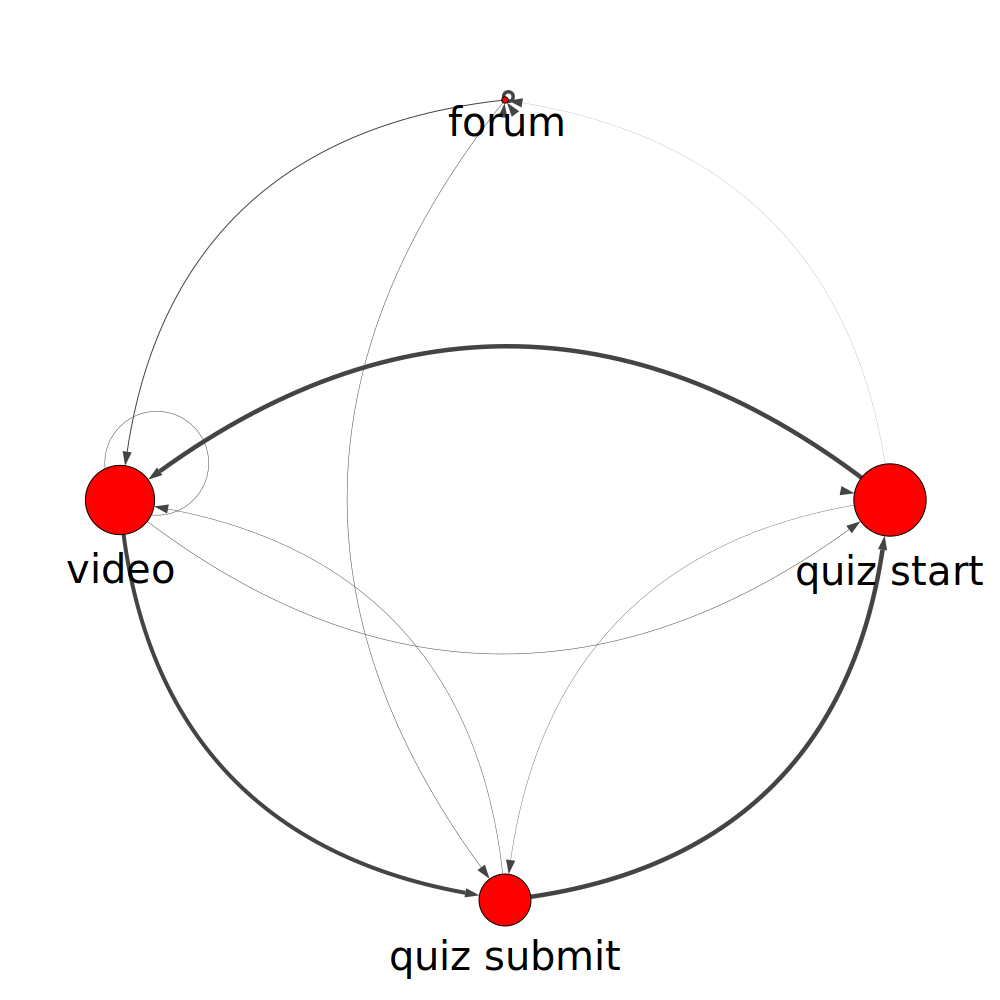
\includegraphics[width=\textwidth]{figures/example/state0.png}
    \caption{Behavior pattern 0\label{fig:motivating-example-0}}
  \end{subfigure}
  \begin{subfigure}[t]{0.30\textwidth}
    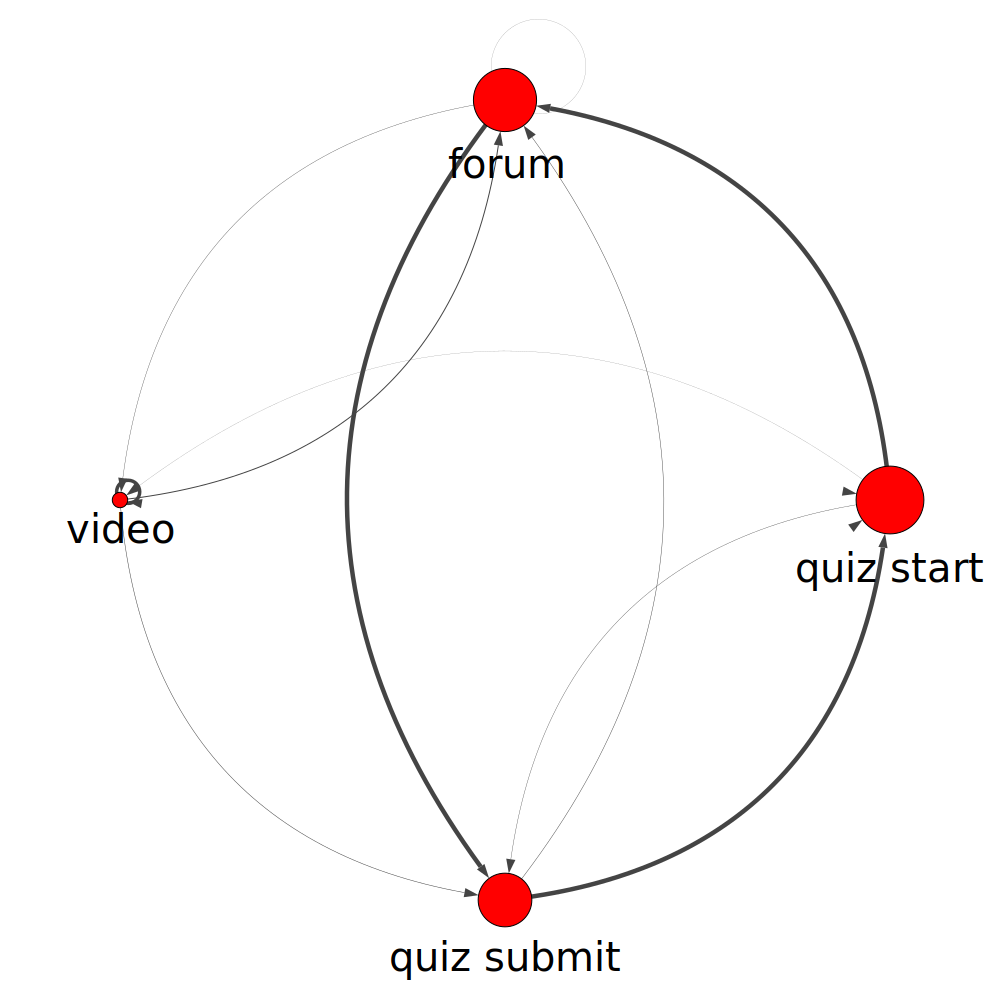
\includegraphics[width=\textwidth]{figures/example/state1.png}
    \caption{Behavior pattern 1\label{fig:motivating-example-1}}
  \end{subfigure}
  \begin{subfigure}[t]{0.30\textwidth}
    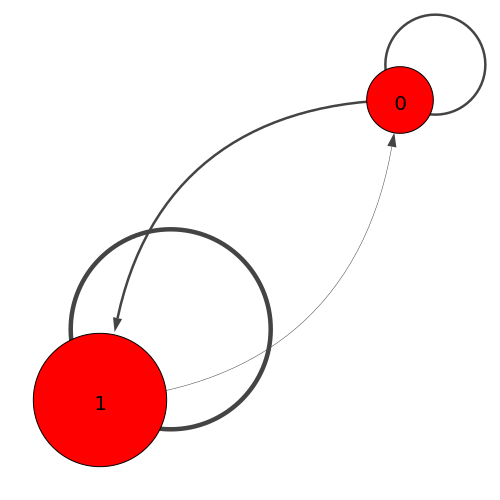
\includegraphics[width=\textwidth]{figures/example/trans.png}
    \caption{Transitions between the two behavior patterns to the
    left.\label{fig:motivating-example-trans}}
  \end{subfigure}
  \caption{An idealized example of what our behavior representation could capture.}
  \label{fig:motivating-example}
\end{figure}
We could infer many things from even such a simple example. The first might
be that, when students are taking quizzes, they tend to either use the
forum or the videos for support, but not both. They also tend to take
quizzes in a sort of ``cycle'' pattern, indicating perhaps that this course
allows quiz re-takes. Finally, in Figure~\ref{fig:motivating-example-trans}
we could conclude that users tend to change their quiz-taking behavior over
time from one that is more video-focused (pattern 0) to one that is more
forum-focused (pattern 1).

Our goal in this paper is to design a model that can automatically capture
student behavior in this way via unsupervised learning methods applied to
large collections of click logs associated with MOOCs. We view our model
as a component of a system that enables collaboration between the machine
and a human instructor to extract knowledge from these large collections of
MOOC data. Automatically extracting interpretable patterns from the
clickstream data associated with MOOCs is a necessary step in order for
instructors to identify the hidden knowledge in these massive interaction
datasets. Without the availability of a suitable model for identifying
these behavioral patterns, instructors are not empowered to use this
available data to improve their courses without expending extraordinary
amounts of manual effort.

Our proposed model is motivated by the following observations:
\begin{enumerate}
  \item Student behavior is complicated and cannot necessarily be captured
      sufficiently by rule-based methods such as those explored by
      \citet{Kizilcec:2013:LAK} and \citet{Davis:2016:EDM}. We instead
      propose to treat student behavior patterns as being characterized
      (represented) via a sequence of \emph{latent states}. This allows us
      to automatically capture patterns that we might not have been able to
      articulate clearly a priori via a series of rules, and also allows us
      to model the inherent uncertainty in assigning a student's behavior
      to a particular pattern or group.
  \item Student behavior can vary over time. Previous models that treat students
      as exhibiting only one behavioral pattern over
      time~\cite{Faucon:2016:EDM} miss out on the opportunity to understand
      student behavior dynamics in a course. We propose a latent space
      model with {\em latent state transitions} to flexibly model the
      dynamics.
  \item Analysis of student behavior can and should be performed at varying
      levels of granularity. This requires us to aggregate data over time
      with \emph{different levels of resolution}; existing models tend to come
      with a particular assumption about the resolution of time they
      consider~\cite{Faucon:2016:EDM, Kizilcec:2013:LAK, Shih:2010:EDM}. We
      propose a model that is agnostic to the time resolution considered,
      allowing it to be applied at different levels of resolution more
      naturally.
\end{enumerate}

Thus, what we propose is a \emph{latent variable approach} to mining student behavior
patterns that is \emph{probabilistic} for inference and
does \emph{not} force assumptions about time resolutions, making it
\emph{flexible to model state changes over different time resolutions} more
easily.  More specifically, we propose a novel two-layer hidden Markov
model (2L-HMM) to discover latent student behavior patterns via
unsupervised learning on large collections of student behavior observation
sequences.  Evaluation results on a MOOC data set on Coursera demonstrate
that the 2L-HMM can effectively discover a variety of interesting interpretable
student behavior patterns at different levels of resolution, many of which
are beyond what existing approaches can discover. We show that the patterns
uncovered by the 2L-HMM capture meaningful behavior by quantitatively
showing that features extracted from a trained 2L-HMM correlate with
learning outcomes. Since our proposed methods are
unsupervised, they can potentially be applied to any MOOC data without
requiring manual annotation effort at the level of sequences. Instead,
instructors are empowered to use the latent patterns that the 2L-HMM can
discover from raw data to extract knowledge about the behaviors his/her
students exhibit in the MOOC.
